\documentclass{article}

\usepackage{arxiv}

\usepackage[utf8]{inputenc} % allow utf-8 input
\usepackage[T1]{fontenc}    % use 8-bit T1 fonts
\usepackage[hidelinks]{hyperref}       % hyperlinks
\usepackage{url}            % simple URL typesetting
\usepackage{booktabs}       % professional-quality tables
\usepackage{amsmath,amssymb,amsthm}
\usepackage{amsfonts}       % blackboard math symbols
\usepackage{nicefrac}       % compact symbols for 1/2, etc.
\usepackage{microtype}      % microtypography
\usepackage{mathrsfs}
\usepackage{graphicx}
\usepackage{doi}
\usepackage{acronym}
\usepackage{listings}
\usepackage{tikz}

\usetikzlibrary{trees}

\newacro{abm}[ABM]{Agent-Based Model}
\newacro{cabm}[CABM]{Cellular Agent-Based Model}
\newacro{ca}[CA]{Cellular Automaton}
\newacroplural{ca}[CA]{Cellular Automata}

\title{
    Mathematical Foundations of\\
    Cellular Agent-Based Models
}

%\date{September 9, 1985}	% Here you can change the date presented in the paper title
%\date{} 					% Or removing it

\author{
    \href{https://orcid.org/0009-0001-0613-7978}{
        
\includegraphics[scale=0.06]{orcid.pdf}
        \hspace{1mm}Jonas Pleyer
    }
    \thanks{
        \href{https://jonas.pleyer.org}{jonas.pleyer.org},
        \href{https://cellular-raza.com}{cellular-raza.com}
    }\\
	Freiburg Center for Data-Analysis and Modeling\\
	University of Freiburg\\
	\texttt{jonas.pleyer@fdm.uni-freiburg.de} \\
	%% examples of more authors
	\And
	\href{https://orcid.org/0000-0002-6371-4495}{
        
\includegraphics[scale=0.06]{orcid.pdf}
        \hspace{1mm}Christian Fleck
    }\\
	Freiburg Center for Data-Analysis and Modeling\\
	University of Freiburg
}

% Uncomment to remove the date
%\date{}

% Uncomment to override  the `A preprint' in the header
\renewcommand{\headeright}{Preprint}
%\renewcommand{\undertitle}{Technical Report}
\renewcommand{\shorttitle}{Mathematical Foundations of Cellular Agent-Based Models}

%%% Add PDF metadata to help others organize their library
%%% Once the PDF is generated, you can check the metadata with
%%% $ pdfinfo template.pdf
\hypersetup{
pdftitle={Mathematical Foundations of Cellular Agent-Based Models},
pdfsubject={q-bio.NC, q-bio.QM},
pdfauthor={Jonas Pleyer, Christian Fleck},
pdfkeywords={},
}

% Define definition, example, lemma, proof and theorem.
\newtheorem{definition}{Definition}[section]
\newtheorem{example}[definition]{Example}
\newtheorem{lemma}[definition]{Lemma}
\newtheorem{theorem}[definition]{Theorem}

% Change numbering of equations
% \numberwithin{equation}{section}

% MAKE TITLES IN THEOREMS BOLD
\makeatletter
\def\th@plain{%
  \thm@notefont{}% same as heading font
  \itshape % body font
}
\def\th@definition{%
  \thm@notefont{}% same as heading font
  \normalfont % body font
}
\makeatother

\begin{document}
\maketitle

\begin{abstract}
\end{abstract}


% keywords can be removed
\keywords{Agent-Based \and Cell \and Biology \and Dynamical System}


\section{Introduction}
\label{sec:introduction}
Over the course of the last decades, many cellular \acp{abm} have been proposed and implemented
\cite{PoncedeLeon2022,Hoehme2010,Lupperger2020}.
Their puposes range from early embryogenesis to cancer research over to wound
healing~\cite{Ziraldo2013}.
Some of these models provide exact mathematical formulations \cite{Ghaffarizadeh2018,Tanaka2015} of
the system which they solve.
Although it is well-known that \acp{abm} and \acp{ca} are a subclass of (continous or discrete)
dynamical systems \cite{Wolfram1984} there has not yet been a directed effort towards a unifying
mathamtical formalism for \acp{cabm}.
We aim to provide insights into a variety of shared concepts along specific examples with real
use-cases.
We construct this formalism along the implementation of our numerical simulation framework
\lstinline{cellular_raza}~\cite{Pleyer_cellular_raza_2024}.

\acp{abm} are centered around the thought that cells are the fundamental building-blocks of nature.
Every cellular agent is distinct to any other and can in principle be tracked throughout space and
time.
The individual behaviour of cells results in the emergence of global phenomena such as spatial or
temporal patterns \cite{Owen2020,Wolpert1969,Giudicelli2007}.
The cells are part of the physical domain and may interact with it in various ways eg. via exchange
of Ligands or physical forces.
Furthermore, cells interact with each other directly.
Most of these interactions are of short range compared to the total size of the system although
counter-examples such as electrical signals exist \cite{Ded2021}.
We explicitly note that our assumptions are not fundamental and loosening of these restrictions can
be discussed to possibly cover a wider variety of problems.
It is important to consider these limitations when applying this theoretical framework.

\section{The Cellular Space $\mathscr{C}$}
We assume that each individual cell lives in a set $C$ which describes all possible configurations
of this single cell.
Cellular systems are characterized by the fact that cells are in principle (although in
practice sometimes more difficult) tracable through time and space.
Depending on the cellular representation we might encounter two cells with identical parameters and
properties (eg. position, intracellular concentrations) which are still distinct agents and can not
be interchanged arbitrarily.
This case could occur eg. when representing cellular positions by whole numbers as in a
\ac{ca}.
This point is further made clear when thinking about cellular proliferation as a tree.
Figure~\ref{fig:cell-lineage-break} shows a hypothetical change between two child-cells.
If we would interchange child $c_{12}$ with $c_{21}$, this would mean that two grandchild-cells
$gc_{212}$ and $gc_{221}$ would have different grandparent-cells.

\begin{figure}
    \centering
    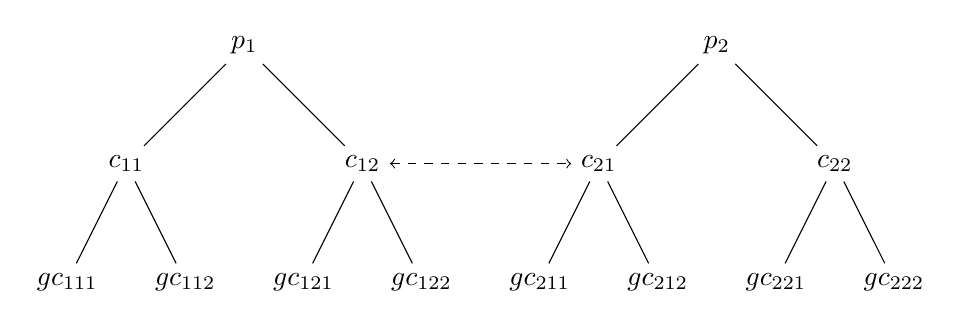
\begin{tikzpicture}[level distance=1.5cm,
      level 1/.style={sibling distance=3cm},
      level 2/.style={sibling distance=1.5cm}]
      \node {$p_1$}
        child {node {$c_{11}$}
          child {node {$gc_{111}$}}
          child {node {$gc_{112}$}}
        }
        child {node (c12) {$c_{12}$}
        child {node {$gc_{121}$}}
          child {node {$gc_{122}$}}
        };
        \node[] at (6, 0) {$p_2$}
        child {node (c21) {$c_{21}$}
          child {node {$gc_{211}$}}
          child {node {$gc_{212}$}}
        }
        child {node {$c_{22}$}
        child {node {$gc_{221}$}}
          child {node {$gc_{222}$}}
        };
        \draw[dashed,<->] (c12) -- (c21);
    \end{tikzpicture}
    \caption{
        Arbitrary cells can not be interchanged freely since this might introduce incorrect
        configurations into the cell-lineage.
        For example, the two cousin-cells $gc_{212}$ and $gc_{221}$ would have different
        grandparent-cells if $c_{12}$ and $c_{21}$ would be interchanged.
    }
    \label{fig:cell-lineage-break}
\end{figure}

This exemplifies the need to assign unique identifiers for cells to correctly trace their lineage.
We call the set of all identifiers $J$ and only consider cells as a combination of an element
$c\in C$ with an identifier $j\in J$.
Thus a cell is an element of the product $J\times C$.
The explicit representation of $J$ can depend on the respective system in question.

\begin{definition}[Cellular State]
    \label{def:cellular-state}
    Let $J$ be a set of identifiers and $C$ be the set describing cellular agents.
    We call a set of cells $M\in Pot(J\times C)$ a cellular state if $M$ is finite and every cell
    has a unique identifer ie. $\#\pi_1(M)=\#M$.
\end{definition}

To allow for processes such as cell-division and death we additionally must be able to treat a
variable number of cells throughout the evolution of the dynamical system.
The evolution function of our dynamical system will map cellular states onto each other, thus
acting on the cellular space $\mathscr{C}$.

\begin{definition}[Cellular Space]
    \label{def:cellular-space}
    The cellular space $\mathscr{C}(J, C)$ of an index set $J$ and cellular configuration space $C$
    is given by $\mathscr{C}(J,C) = \{M\in Pot(J\times C) | M \text{ is cellular state }\}$.
    We may choose the simplified notation $\mathscr{C} = \mathscr{C}(J, C)$ where the context is
    clear.
\end{definition}

Furthermore, as can be seen from Figure~\ref{fig:cell-lineage-break}, division of cells introduces
two new identifiers with two new cells and consumes the previously existing cell.
Cell-death removes cells but newly created ones may not obtain their unique identifier making it
also unique in time.

\begin{definition}[Cell Division]
    TODO proliferation
\end{definition}
\begin{definition}[Cell Death]
    TODO
    - apoptosis
    - necrosis
    - removal
\end{definition}

\begin{lemma}[Cellular Identity]
    \label{thm:cellular-uniqueness}
    Given an index $j\in J$, we define the set of time-points $T_j=\{t\in T: j\in\phi_t(x_0)\}$.
    Let the underlying time monoid $T$ of our \ac{abm} be a connected topological space.
    a path-connected subset
    $U\subset T$ where $T$ is the monoid of our dynamical system describing time.
\end{lemma}
\begin{proof}
    TODO
\end{proof}

\section{Dynamics}
\begin{definition}[Dynamical System]
    A dynamical system is a tuple $(T,M,\phi)$ where $T$ is a monoid (written additively) and
    $\phi$ is a mapping
    \begin{equation}
        \phi : U\subset(T\times M) \rightarrow M
    \end{equation}
    with $\pi_2(U) = M$ where $\pi_2$ is the projection on the second coordinate and $\phi$
    satisfies
    \begin{align}
        \phi(0,m) &= m\\
        \phi(t_2, \phi(t_1, m)) &= \phi(t_2+t_1,m).
    \end{align}
\end{definition}
We often write $\phi(t,m) = \phi_t(m)$.
Classical \acp{ca} such as Conway's Game of Life \cite{Graner1992} or the Cellular Potts Model
\cite{games1970fantastic} are spatially and temporally discrete dynamical systems.
In the case of \acp{abm} the space $M$ consists of the collection of all currently living cells
$\mathscr{C}$ and the physical domain $D$ in which they live ie. $M=\mathscr{C}\times D$.

\begin{example}[Game of Life]
    \label{example:game-of-life}
    Conway's Game of Life is perhaps the most popular example for a cellular automaton.
    It is deterministic and acts on a infinite grid $\mathbb{Z}^2$ by assigning one of two states
    (alive or dead) to each grid-point
    \begin{equation}
        L:\mathbb{Z}^2\rightarrow\{0,1\}
    \end{equation}
    where we prefer the short-hand notation $L(i,j)=L_{ij}$ or $L^n_{ij}$ where $n$ is the temporal
    index.
    This means a single state is described by a mapping $L:\mathbb{Z}^2\rightarrow\{0,1\}$ and the
    evolution function of this dynamical system acts on the space of these maps
    $X:=\{L:\mathbb{Z}^2\rightarrow\{0,1\}\}$
    \begin{equation}
        \phi:U\subset(\mathbb{N}\times X) \rightarrow X
    \end{equation}
    where we identified $(\mathbb{N},+)$ as the monoid of the dynamical system.
    Let $\eta_{ij}\subset\mathbb{Z}^2$ be the set of spatial indices which are direct neighbors of
    $(i,j)$ ie. $\eta_{ij}=\{(k,l)\in\mathbb{Z}^2 \text{ where } |k-i|<2, |l-j|<2 \text{ and }
    (k,l)\neq(i,j)\}$.
    The game consists of three rules:
    \begin{enumerate}
        \item Any live cell with fewer than two live neighbors dies, as if by underpopulation.
        \item Any live cell with two or three live neighbors lives on to the next generation.
        \item Any live cell with more than three live neighbors dies, as if by overpopulation.
        \item Any dead cell with exactly three live neighbors becomes a live cell, as if by
            reproduction.
    \end{enumerate}
    Together with the sum of all neighboring cells $S_{ij}=\sum\limits_{\iota\in\eta_{ij}}L^n_\iota$
    we can write these as
    \begin{equation}
        \phi_1(L_{ij}^n) = L_{ij}^{n+1} =
        \begin{cases}
            0 &L^n_{ij}=1 \text{ and } S_{ij}<2\\
            1 &L^n_{ij}=1 \text{ and } S_{ij}=2,3\\
            0 &L^n_{ij}=1 \text{ and } S_{ij}>3\\
            1 &L^n_{ij}=0 \text{ and } S_{ij}=3\\
            0 &\text{else}
        \end{cases}
    \end{equation}
    which fully specifies the dynamical system when applying iteratively
    $\phi_m=\phi_1\circ\dots\circ\phi_1$.
\end{example}

When we compare the above rules with definitions~\ref{def:cellular-state}
and~\ref{def:cellular-space}, we immediately see that the cellular identity is not preserved for the
4th rule.
This \ac{ca} assumes that a new cell is created from 3 neighboring cells which is contrary to the
division process of cells.
We set out to formualte the Game of Life within the framework of cellular \acp{abm}.
To circumvent this problem, we could assume that simply one of the present cells divides and is
chosen randomly with even probability.
In order to formalize such a system we would require to introduce the notion of a
Stochastic Dynamical System.
But this raises the problem that the second cell of this division process would have to also be
inserted somewhere in the \ac{ca}.
Asked in more general terms: Given an arbitrary state $L^n_{ij}$:
Is it possible to describe a single transition $L^n_{ij}\rightarrow L^{n+1}_{ij}$ by a combination
of finitely many cellular division and death processes?
In general: No.
This is made clear by considering the example of Figure~\ref{fig:conway-non-abm-transition}.
The transition shown can not be described by any combination of division and death under the
consideration that cell-death can only act on currently alive cells.
In principle, this conundrum could be lifted when performing the division and death process in
different steps but this would change the outcome and behaviour of the system.
Similarly, other \acp{ca} such as the Cellular Potts Model~\cite{Graner1992} or Rule
184~\cite{Krug1988} can not
directly be translated into an \ac{cabm}.
This shows that even the fundamental choices in the design of \acp{cabm} already present interesting
restrictions and \acp{ca} should in general not be treated as special cases of \acp{cabm}.

\begin{figure}
    \centering
    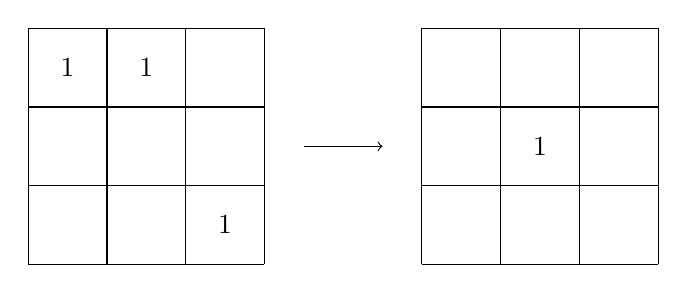
\begin{tikzpicture}
        \draw (0,0) -- (3,0);
        \draw (0,0) -- (0,3);
        \draw (3,0) -- (3,3);
        \draw (0,3) -- (3,3);
        \draw (1,0) -- (1,3);
        \draw (2,0) -- (2,3);
        \draw (0,1) -- (3,1);
        \draw (0,2) -- (3,2);
        \node at (2.5,0.5) {1};
        \node at (0.5,2.5) {1};
        \node at (1.5,2.5) {1};
        \draw[->] (3.5,1.5) -- (4.5,1.5);
        \draw (0+5,0) -- (3+5,0);
        \draw (0+5,0) -- (0+5,3);
        \draw (3+5,0) -- (3+5,3);
        \draw (0+5,3) -- (3+5,3);
        \draw (1+5,0) -- (1+5,3);
        \draw (2+5,0) -- (2+5,3);
        \draw (0+5,1) -- (3+5,1);
        \draw (0+5,2) -- (3+5,2);
        \node at (1.5+5,1.5) {1};
    \end{tikzpicture}
    \caption{
        This transition in Conways Game of Life can not be described by any combination of
        cell-division and death.
        The cell in the middle which is being created by rule 4 is new and must thus be created by
        the division mechanism in our \ac{abm}.
        If any of the initial cells divide, we obtain 2 new cells which need to placed.
        Since cell-death can only affect currently existing cells, this is contradictory to the
        final state which only contains a single cell.
    }
    \label{fig:conway-non-abm-transition}
\end{figure}

\section{Dynamics}

\section{Spatial Decomposition}
We assume that the physical domain $D$ can be split into smaller subdomains
$\bigcup_{i\in I}S_i=D$ which are pairwise disjoint.
We will later require that any dynamics can be calculated by considering cellular agents inside a
given subdomain $S_i$ and their interactions with neighboring subdomains.
This also applies to spatial effects such as diffusion.
Therefore, we must first develop the notion of being a \textbf{neighbor}.

\begin{definition}[Neighbor]
    The notion of neighbor can be defined by two equivalent methods.
    \begin{enumerate}
        \item We call $\eta:I\rightarrow Pot(I)$ a \textbf{neighbor map} if
        \item $i\in\eta(j) \Leftrightarrow j\in\eta(i)$ for each $i,j\in I$.
            We call a relation $||$ on $I$ a \textbf{neighbor relation} if it is symmetric.
    \end{enumerate}
\end{definition}

\begin{example}[Moore Neighbors]
    The neighborhood used in the Game of Life~\ref{example:game-of-life} is the 2-dimensional
    special case.
    In general, for any discrete space $\mathbb{Z}^n$, we consider the Moore neighborhood $U(x)$ for
    any point $x\in\mathbb{Z}^n$ to be
    \begin{equation}
        U(x) := \{y\in\mathbb{Z}^n:\max\limits_{i=1}^n|x_i-y_i|=1\}.
    \end{equation}
    This definition ensures that at least one component of the value $y$ is not identical to the
    point in question $x$.
    This metric is also often called uniform norm, supremum norm (in a possibly infinite-dimensional
    case) or Chebyshev norm~\cite{Rudin1976}.
\end{example}

Note that in the numerical implementation it is often more convenient to work with the first
definition while the second can be more useful in a theoretical context.

\begin{proof}
    $1) \Rightarrow 2)$ Let $\eta$ be a neighbor map.
    We define a relation $||$ by $i||j \Leftrightarrow i\in\eta(j)$.
    It is clear that $||$ is symmetric.\\
    $2) \Rightarrow 1)$ Let $||$ be a symmetric relation on $I$.
    We define the function $\eta:I\rightarrow Pot(I)$ via
    $\eta(i):=\{j\in I \text{ such that } i||j\}$.
    If $j\in\eta(i)$ then $i||j \Leftrightarrow j||i$ and thus $i\in\eta(j)$.
\end{proof}

Equipped with this notion of \textbf{neighbor}, we can now formalize the spatial splitting of our
domain.

\begin{definition}[Spatial Decomposition]
    A Spatial Decomposition of a domain $D$ is a collection of subsets
    $\{S_i\subset D: i\in I\}$ together with a either a neighbor map $\eta$ or neighbor relation
    $||$ such that $D=\cup_{i\in I}$ and $S_i$ are pairwise disjoint.
\end{definition}

\subsection{Properties of Multicellular Systems}
\label{subsec:introduction-properties}

\begin{enumerate}
    \item Stochastic -> Irreversible
    \item Dissipative (take up energy, non-equilibrium, decrease entropy)
\end{enumerate}


\subsection{Individual-Based Descriptions of Cellular Agent}
\label{subsec:introduction-individual-descriptions}

\begin{table}
	\caption{Aspects of cellular systems}
	\centering
	\begin{tabular}{ll}
		% \multicolumn{2}{c}{Part}                   \\
		% \cmidrule(r){1-2}
		\toprule
        Aspect                  &Examples\vspace{0.5em}\\
        \it{(C) Cellular}\\
        \midrule
        Spatial Representation  &elongated rods, soft spheres, vertex-like\\
        Intracellular Forces    &hexagonal shape\\
        Intracellular Reactions &signalling pathways,stress response\\
        Movement                &neighbour exchange, motility, chemotaxis, directed random walk\\
        Cycle                   &differentiation, division, (phased) death, mesenchymal-epithelial transition\vspace{0.5em}\\
        \it{(CC) Cell-Cell Interactions}\\
		\midrule
        Interaction Forces      &adherent forces, friction, de-adhesion\\
        Reactions via Contact   &communication between plant-cells via plasmodesmata, gap-junctions\\
        Neighbour sensing       &phenomenological abstraction\\
        Fusion                  &homotypic, heterotypic\vspace{0.5em}\\
        \it{(DC) Domain-Cell Interactions}\\
        \midrule
        External Forces         &blood flow, microfluidic devices\\
        Boundary Effects        &reflection at petri-dish surface, containment of ligands, adhesion\\
        Extracellular Processes &diffusion of morphogens, transport of signalling molecules\vspace{0.5em}\\
        \it{(O) Other}\\
        \midrule
        External Controller     &introduce drug, remove cells, refresh nutrients\\
		\bottomrule
	\end{tabular}
	\label{tab:table}
\end{table}

\newpage
\pagebreak

\section{Motivation}
\label{subsec:motivation}
In the previous section, we have determined aspects of cellular systems which we aim to describe
with suitable abstractions.
As we have already shown, these aspects can be grouped into 3 categories.
The first category only considers a single cell by itself while the second and third consider
interactions with other cells and the external environment respectively.
Lastly, we allow an external controller to make changes to the experimental setup in accordance with
the experimental reality.

\subsection{Intracellular Representations and Processes}
\label{subsec:abstractions-cell}
\subsubsection{Mechanics - Spatial Representation, Intracellular Forces \& Movement}
\label{subsubsec:abstractions-cell-mechanics}
\subsubsection{Intracellular Reactions}
\label{subsubsec:abstractions-cell-reactions}
\subsubsection{Cycle}
\label{subsubsec:abstractions-cell-cycle}

\subsection{Cell-Cell Interactions}
\label{subsec:abstractions-cell-cell}
\subsubsection{Forces}
\label{subsec:abstractions-cell-cell-forces}
Forces acting between cells are often described in terms of interaction potentials $V(x_i, x_j)$
where $x_i,x_j$ are the position of two cells.
\begin{equation}
    F_i = \nabla_{x_i}V(x_i, x_j)
\end{equation}
If $V$ only depends on the difference between the two positions $x_i-x_j$, we obtain an
antisymmetric expression in $i,j$.
\begin{align}
    F_i &= \nabla_{x_i}V(x_i-x_j)\\
    &= -\nabla_{x_j}V(x_i-x_j)
\end{align}
However, this assumption is only valid for point-like objects without any additional structure.
Consider the example where a cell is represented by two points $(p_1, p_2)$ which are connected with
a spring of length $l$ and strength $D$.
This may be a simplified model for an elongated bacteria.
We can write down the force contribution from intracellular forces
\begin{align}
    F_{\text{intra},i} = \begin{bmatrix}
        - D (|p_1-p_2|-l)\\
        D (|p_1-p_2|-l)
    \end{bmatrix}
\end{align}
We can assume that the two vertices of one cell $p_{1,i},p_{2,j}$ are interacting with both vertices
of the other.
This reslts in a force term of the form
\begin{align}
    F_{\text{extra},i} &= \begin{bmatrix}
        F(p_{1,i}, p_{1,j}) + F(p_{1,i}, p_{2,j})\\
        F(p_{2,i}, p_{1,j}) + F(p_{2,i}, p_{2,j})
    \end{bmatrix}\\
    F_{\text{extra},j} &= \begin{bmatrix}
        F(p_{1,j}, p_{1,i}) + F(p_{1,j}, p_{2,i})\\
        F(p_{2,j}, p_{1,i}) + F(p_{2,j}, p_{2,i})
    \end{bmatrix}
\end{align}
and thus we can clearly see that $F_{\text{extra},i}\neq - F_{\text{extra},j}$ even if
$F(a,b)=-F(b,a)$.
This means that we have to rely on a method which calculates both the forces acting on cell $i$ and
$j$ simultanously.
To be able to model friction forces (although rare) we additionally take the velocity $v_i$ into
account.
Further, we allow additional information $\sigma_i$ to be exchanged between the cells during their
interaction (ie. species specific).
We take this as the basis for calculating forces between cells.
\begin{equation}
    (F_i, F_j) = F(x_i, x_j, v_i, v_j, \sigma_i, \sigma_j)
\end{equation}

\subsection{Domain-Cell Interactions}
\label{subsec:abstractions-domain-cell}

% \subsection{Citations}
% Citations use \verb+natbib+. The documentation may be found at
% \begin{center}
% 	\url{http://mirrors.ctan.org/macros/latex/contrib/natbib/natnotes.pdf}
% \end{center}
% 
% Here is an example usage of the two main commands (\verb+citet+ and \verb+citep+): Some people thought a thing \citep{kour2014real, hadash2018estimate} but other people thought something else \citep{kour2014fast}. Many people have speculated that if we knew exactly why \citet{kour2014fast} thought this\dots
% 
% \subsection{Figures}
% See Figure \ref{fig:fig1}. Here is how you add footnotes. \footnote{Sample of the first footnote.}
% 
% \begin{figure}
% 	\centering
% 	\fbox{\rule[-.5cm]{4cm}{4cm} \rule[-.5cm]{4cm}{0cm}}
% 	\caption{Sample figure caption.}
% 	\label{fig:fig1}
% \end{figure}
% 
% \subsection{Tables}
% See awesome Table~\ref{tab:table}.
% 
% The documentation for \verb+booktabs+ (`Publication quality tables in LaTeX') is available from:
% \begin{center}
% 	\url{https://www.ctan.org/pkg/booktabs}
% \end{center}
% 
% 
% \begin{table}
% 	\caption{Sample table title}
% 	\centering
% 	\begin{tabular}{lll}
% 		\toprule
% 		\multicolumn{2}{c}{Part}                   \\
% 		\cmidrule(r){1-2}
% 		Name     & Description     & Size ($\mu$m) \\
% 		\midrule
% 		Dendrite & Input terminal  & $\sim$100     \\
% 		Axon     & Output terminal & $\sim$10      \\
% 		Soma     & Cell body       & up to $10^6$  \\
% 		\bottomrule
% 	\end{tabular}
% 	\label{tab:table}
% \end{table}
% 
% \subsection{Lists}
% \begin{itemize}
% 	\item Lorem ipsum dolor sit amet
% 	\item consectetur adipiscing elit.
% 	\item Aliquam dignissim blandit est, in dictum tortor gravida eget. In ac rutrum magna.
% \end{itemize}


\bibliographystyle{IEEEtran}
\bibliography{references}  %%% Uncomment this line and comment out the ``thebibliography'' section below to use the external .bib file (using bibtex) .


%%% Uncomment this section and comment out the \bibliography{references} line above to use inline references.
% \begin{thebibliography}{1}

% 	\bibitem{kour2014real}
% 	George Kour and Raid Saabne.
% 	\newblock Real-time segmentation of on-line handwritten arabic script.
% 	\newblock In {\em Frontiers in Handwriting Recognition (ICFHR), 2014 14th
% 			International Conference on}, pages 417--422. IEEE, 2014.

% 	\bibitem{kour2014fast}
% 	George Kour and Raid Saabne.
% 	\newblock Fast classification of handwritten on-line arabic characters.
% 	\newblock In {\em Soft Computing and Pattern Recognition (SoCPaR), 2014 6th
% 			International Conference of}, pages 312--318. IEEE, 2014.

% 	\bibitem{hadash2018estimate}
% 	Guy Hadash, Einat Kermany, Boaz Carmeli, Ofer Lavi, George Kour, and Alon
% 	Jacovi.
% 	\newblock Estimate and replace: A novel approach to integrating deep neural
% 	networks with existing applications.
% 	\newblock {\em arXiv preprint arXiv:1804.09028}, 2018.

% \end{thebibliography}


\end{document}

